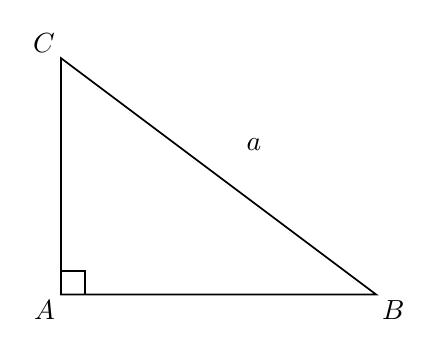
\begin{tikzpicture}[x=1cm,y=1cm,font=\normalsize,
 geometry edge/.style={solid,line width=.6pt},
 geometry mark/.style={solid,line width=.6pt},
 geometry label/.style={font=\normalsize,inner sep=2pt}]
\coordinate (A) at (0,0);
\coordinate (B) at (4,0);
\coordinate (C) at (0,3);
\draw[geometry edge] (A)--(B)--(C)--cycle;
\draw[geometry mark] (0.3,0)--(0.3,0.3)--(0,0.3);
\node[font=\normalsize,inner sep=2pt] at (2.45,1.9) {$a$};
\node[geometry label,below left] at (A) {$A$};
\node[geometry label,below right] at (B) {$B$};
\node[geometry label,above left] at (C) {$C$};
\end{tikzpicture}
